\chapter{Methods}
\section {Study Participants}
We measured 8 normal hearing people. Participant 8 was given silent stimuli as a comparison. The detailed information about the subjects are listed in the table.

\begin{table}[h!]
  \begin{center}
    
    
    \begin{tabular}{p{2.3cm} | p{1.5cm} |p{2.5cm} | p{2.8cm} | p{2.1cm} | p{2.2cm}} % <-- Alignments: 1st column left, 2nd middle and 3rd right, with vertical lines in between
      \textbf{Participant} & \textbf {Gender}& \textbf{Handedness} & \textbf{Race} & \textbf{Hair color} &\textbf {Age (year)}\\ 
      \hline
      1 & F & right-handed & east asian & dark & 22\\
      2 & M & right-handed  & caucasian & blond & 18 \\
      3 & M & left-handed &  caucasian & brunet & 21\\
      4 & F  & right-handed & east asian & dark& 21 \\
      5 & M & right-handed  &  caucasian& blond & 26 \\
      6 &  F & right-handed & southeast asian & dark & 22 \\
      7 &  M & left-handed &  east asian & dark & 23 \\
      8 & M & right-handed  & caucasian & blond & 22 \\
    \end{tabular}
    \label{tab:table1}
    \caption{Demographic information of the study participants.}
  \end{center}
  
\end{table}

\section {Probe Design}
The probes were first designed in AtlasViewer (release v2.11.3 \footnote{\url{https://github.com/BUNPC/AtlasViewer/releases/tag/v2.11.3}})  (see Figure ~\ref{fig:atlas}) \citep {10.1117/1.NPh.2.2.020801} and the SD GUI interface \footnote{a sub GUI of AtlasViewer} (see Figure ~\ref{fig:sdgui}). The probe design was made as close as possible to the research from Weder et al \citeyearpar{Weder2018}. However, several modifications had to be made due to device limitations.

First of all, the paper only provided a rough 2D-sketch of their probe design (see Figure ~\ref{fig:WederProbe}). The channels were not described in detail. Though there are different ways to define the channels, we believe it should not matter as long as the mid-points of the channel correspond to that of the previous research \citep {Weder2018}.

\begin{figure}[H]
  \centering
    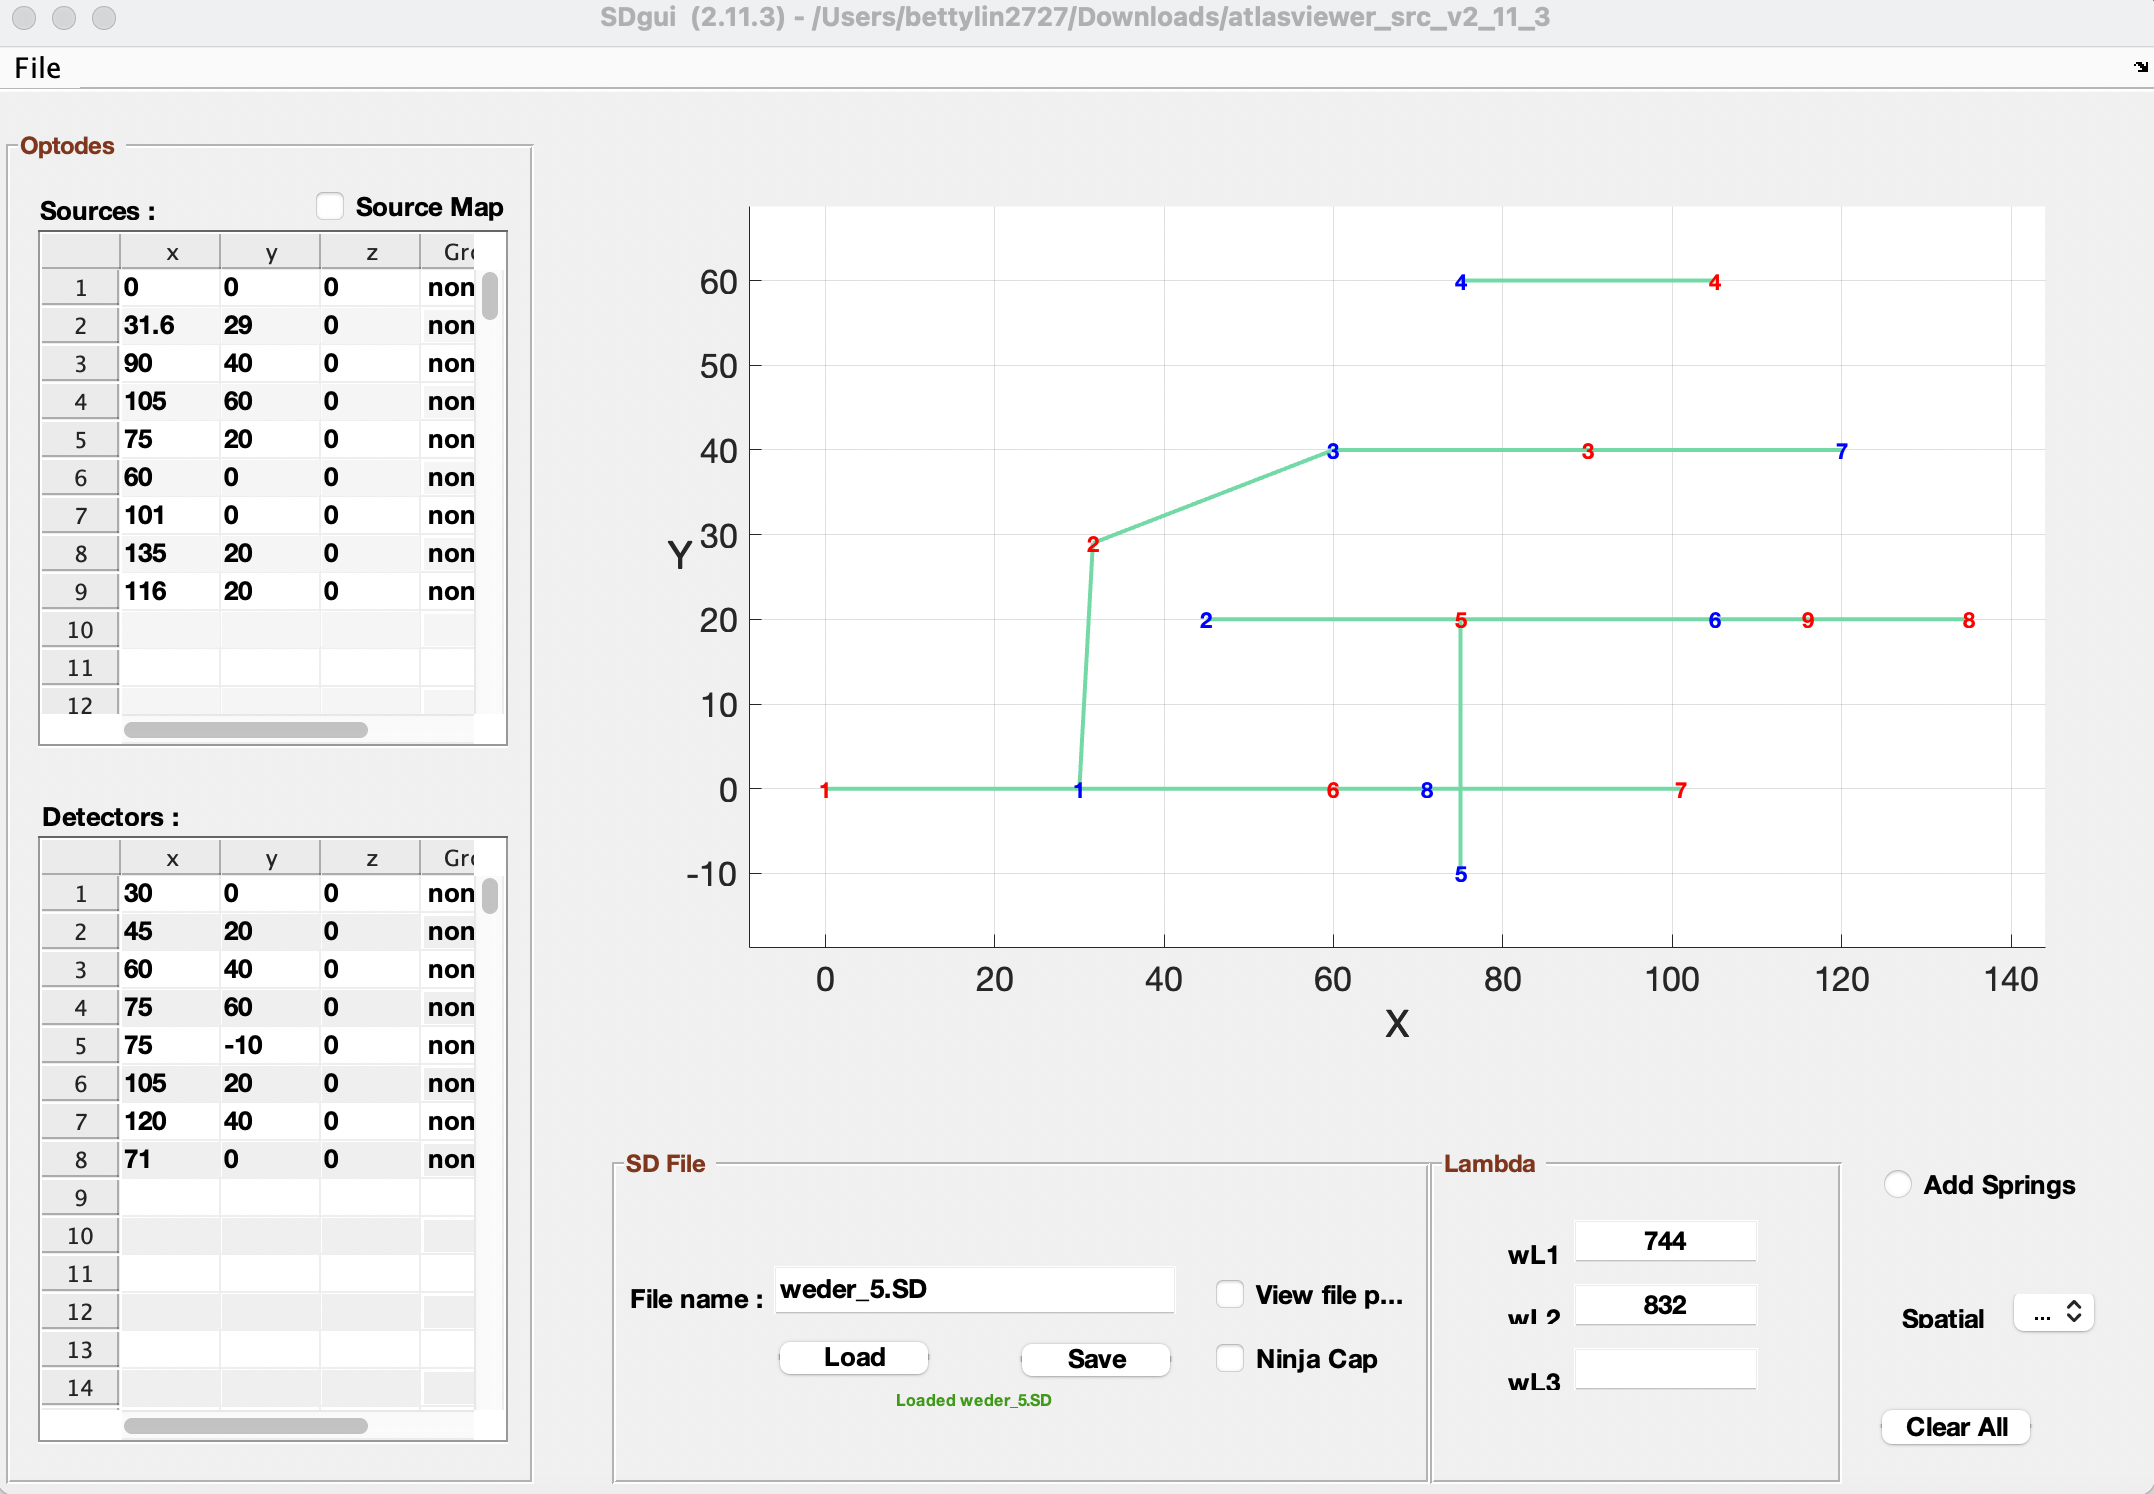
\includegraphics[scale=.35]{bilder/SDgui.png}
  \caption{SDgui interface and optode coordinates.}
  \label{fig:sdgui}
\end{figure}

\begin{figure}[H]
  \centering
  %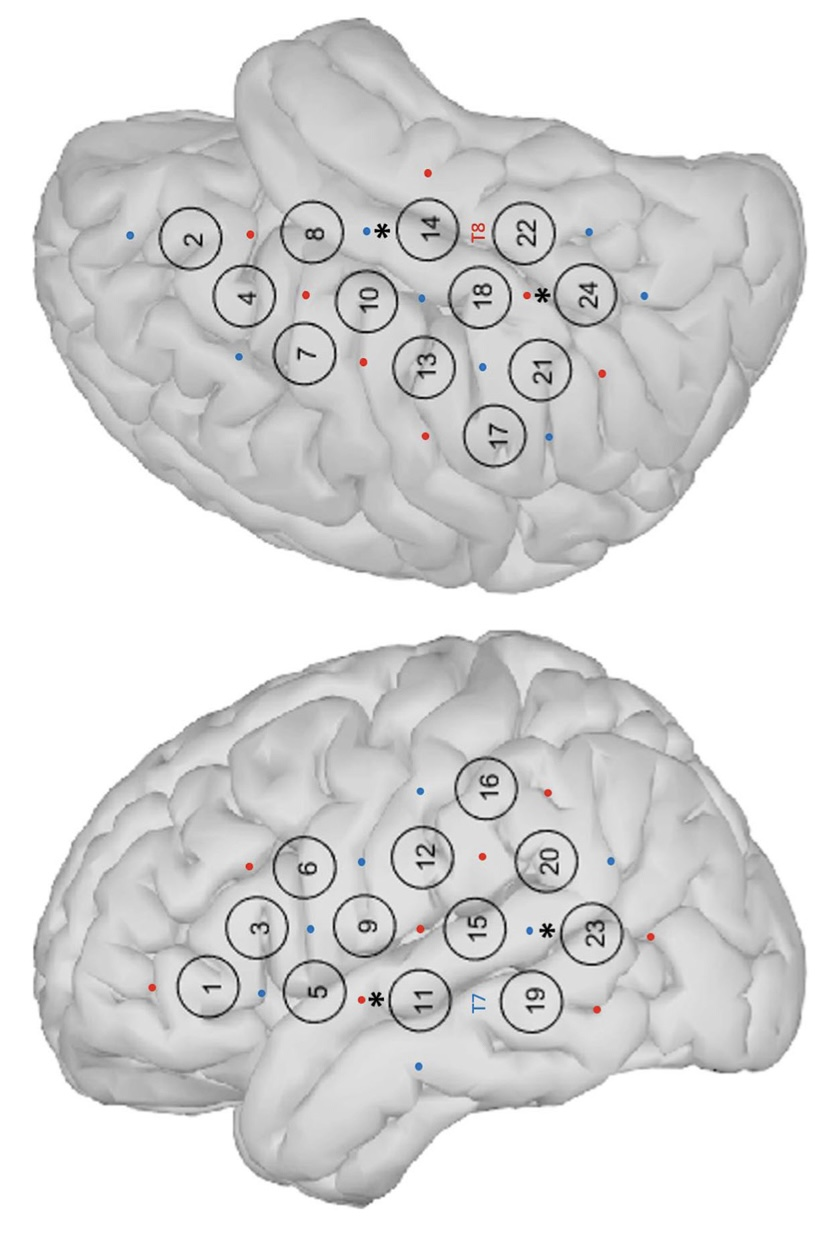
\includegraphics[scale= 0.4]{bilder/weder_probe.jpg}
  \copyrightbox[b]{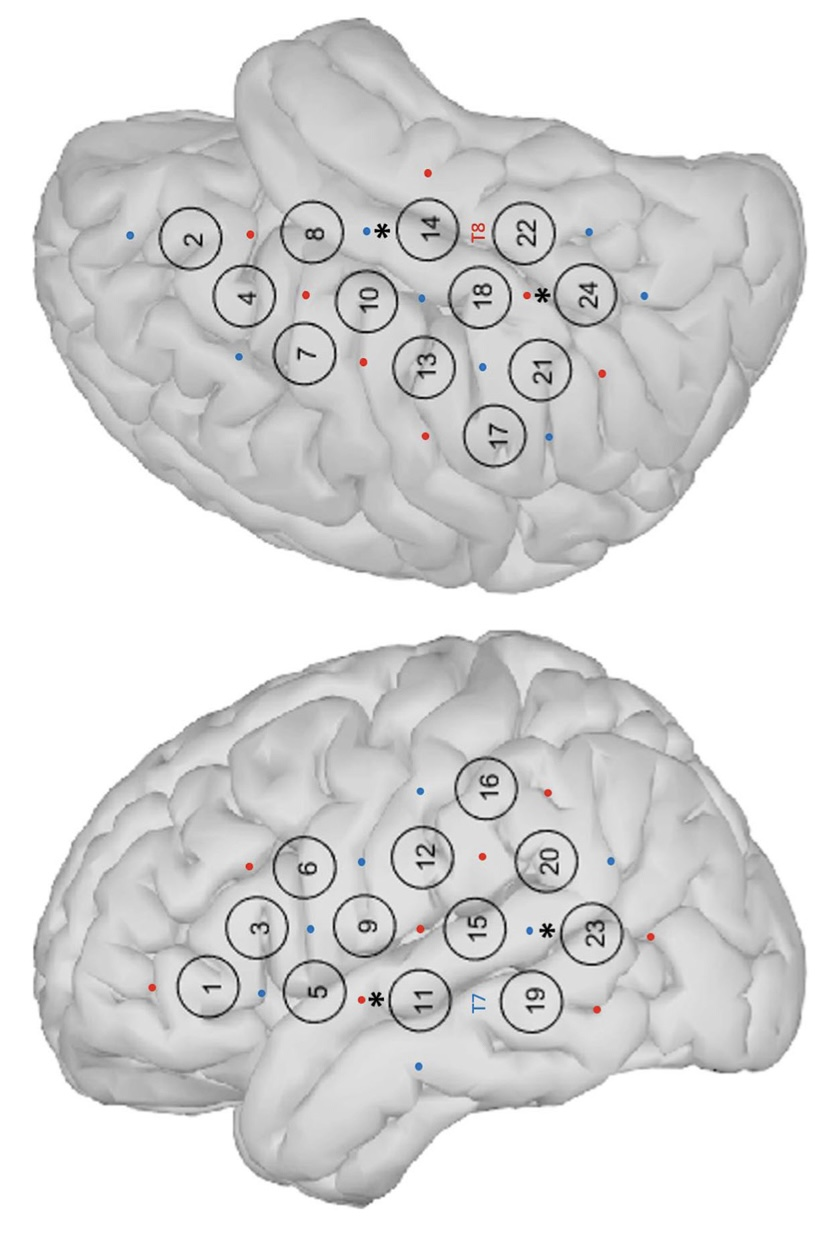
\includegraphics[scale= 0.4]{bilder/weder_probe.jpg}}{Source: \url{https://link.springer.com/article/10.1007/s10162-018-0661-0}}
  \caption{Probe design from Weder et al. \citeyearpar{Weder2018}}
  \label{fig:WederProbe}
\end{figure}

\begin{figure}[H]
  \centering
    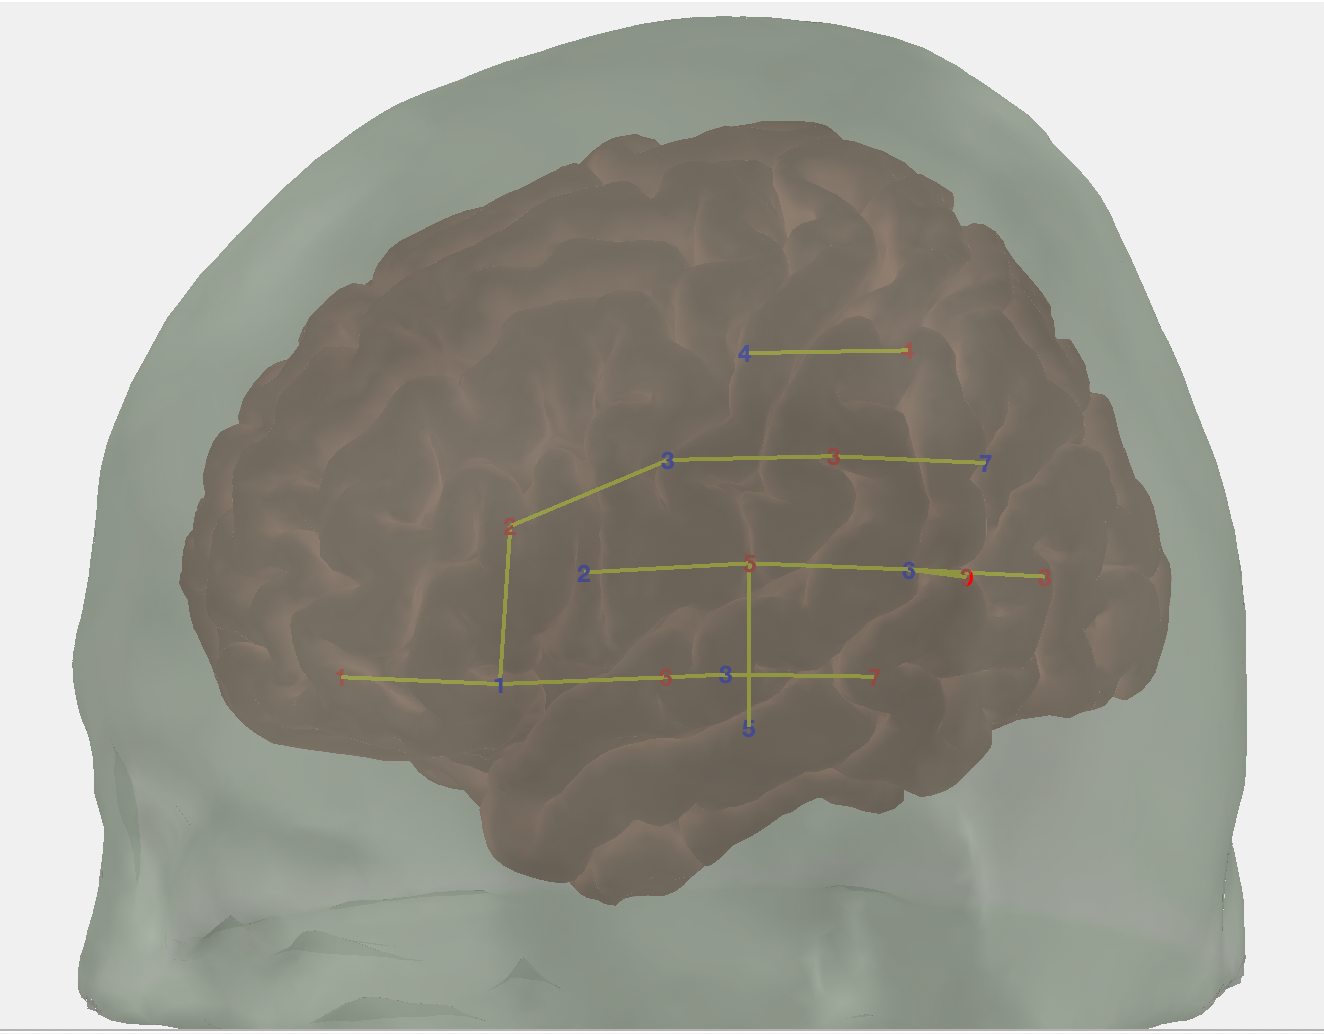
\includegraphics[scale=.35]{bilder/atlas_probe.png}
  \caption{Probe design in this research. Shown in AtlasViewer  \citeyearpar {10.1117/1.NPh.2.2.020801} . The red numbers represent the light sources and the blue numbers represent the dectector. Channels are shown in yellow lines.}
  \label{fig:atlas}
\end{figure}



\begin{figure}
\centering
\begin{minipage}[c]{.4\linewidth}
  \centering
  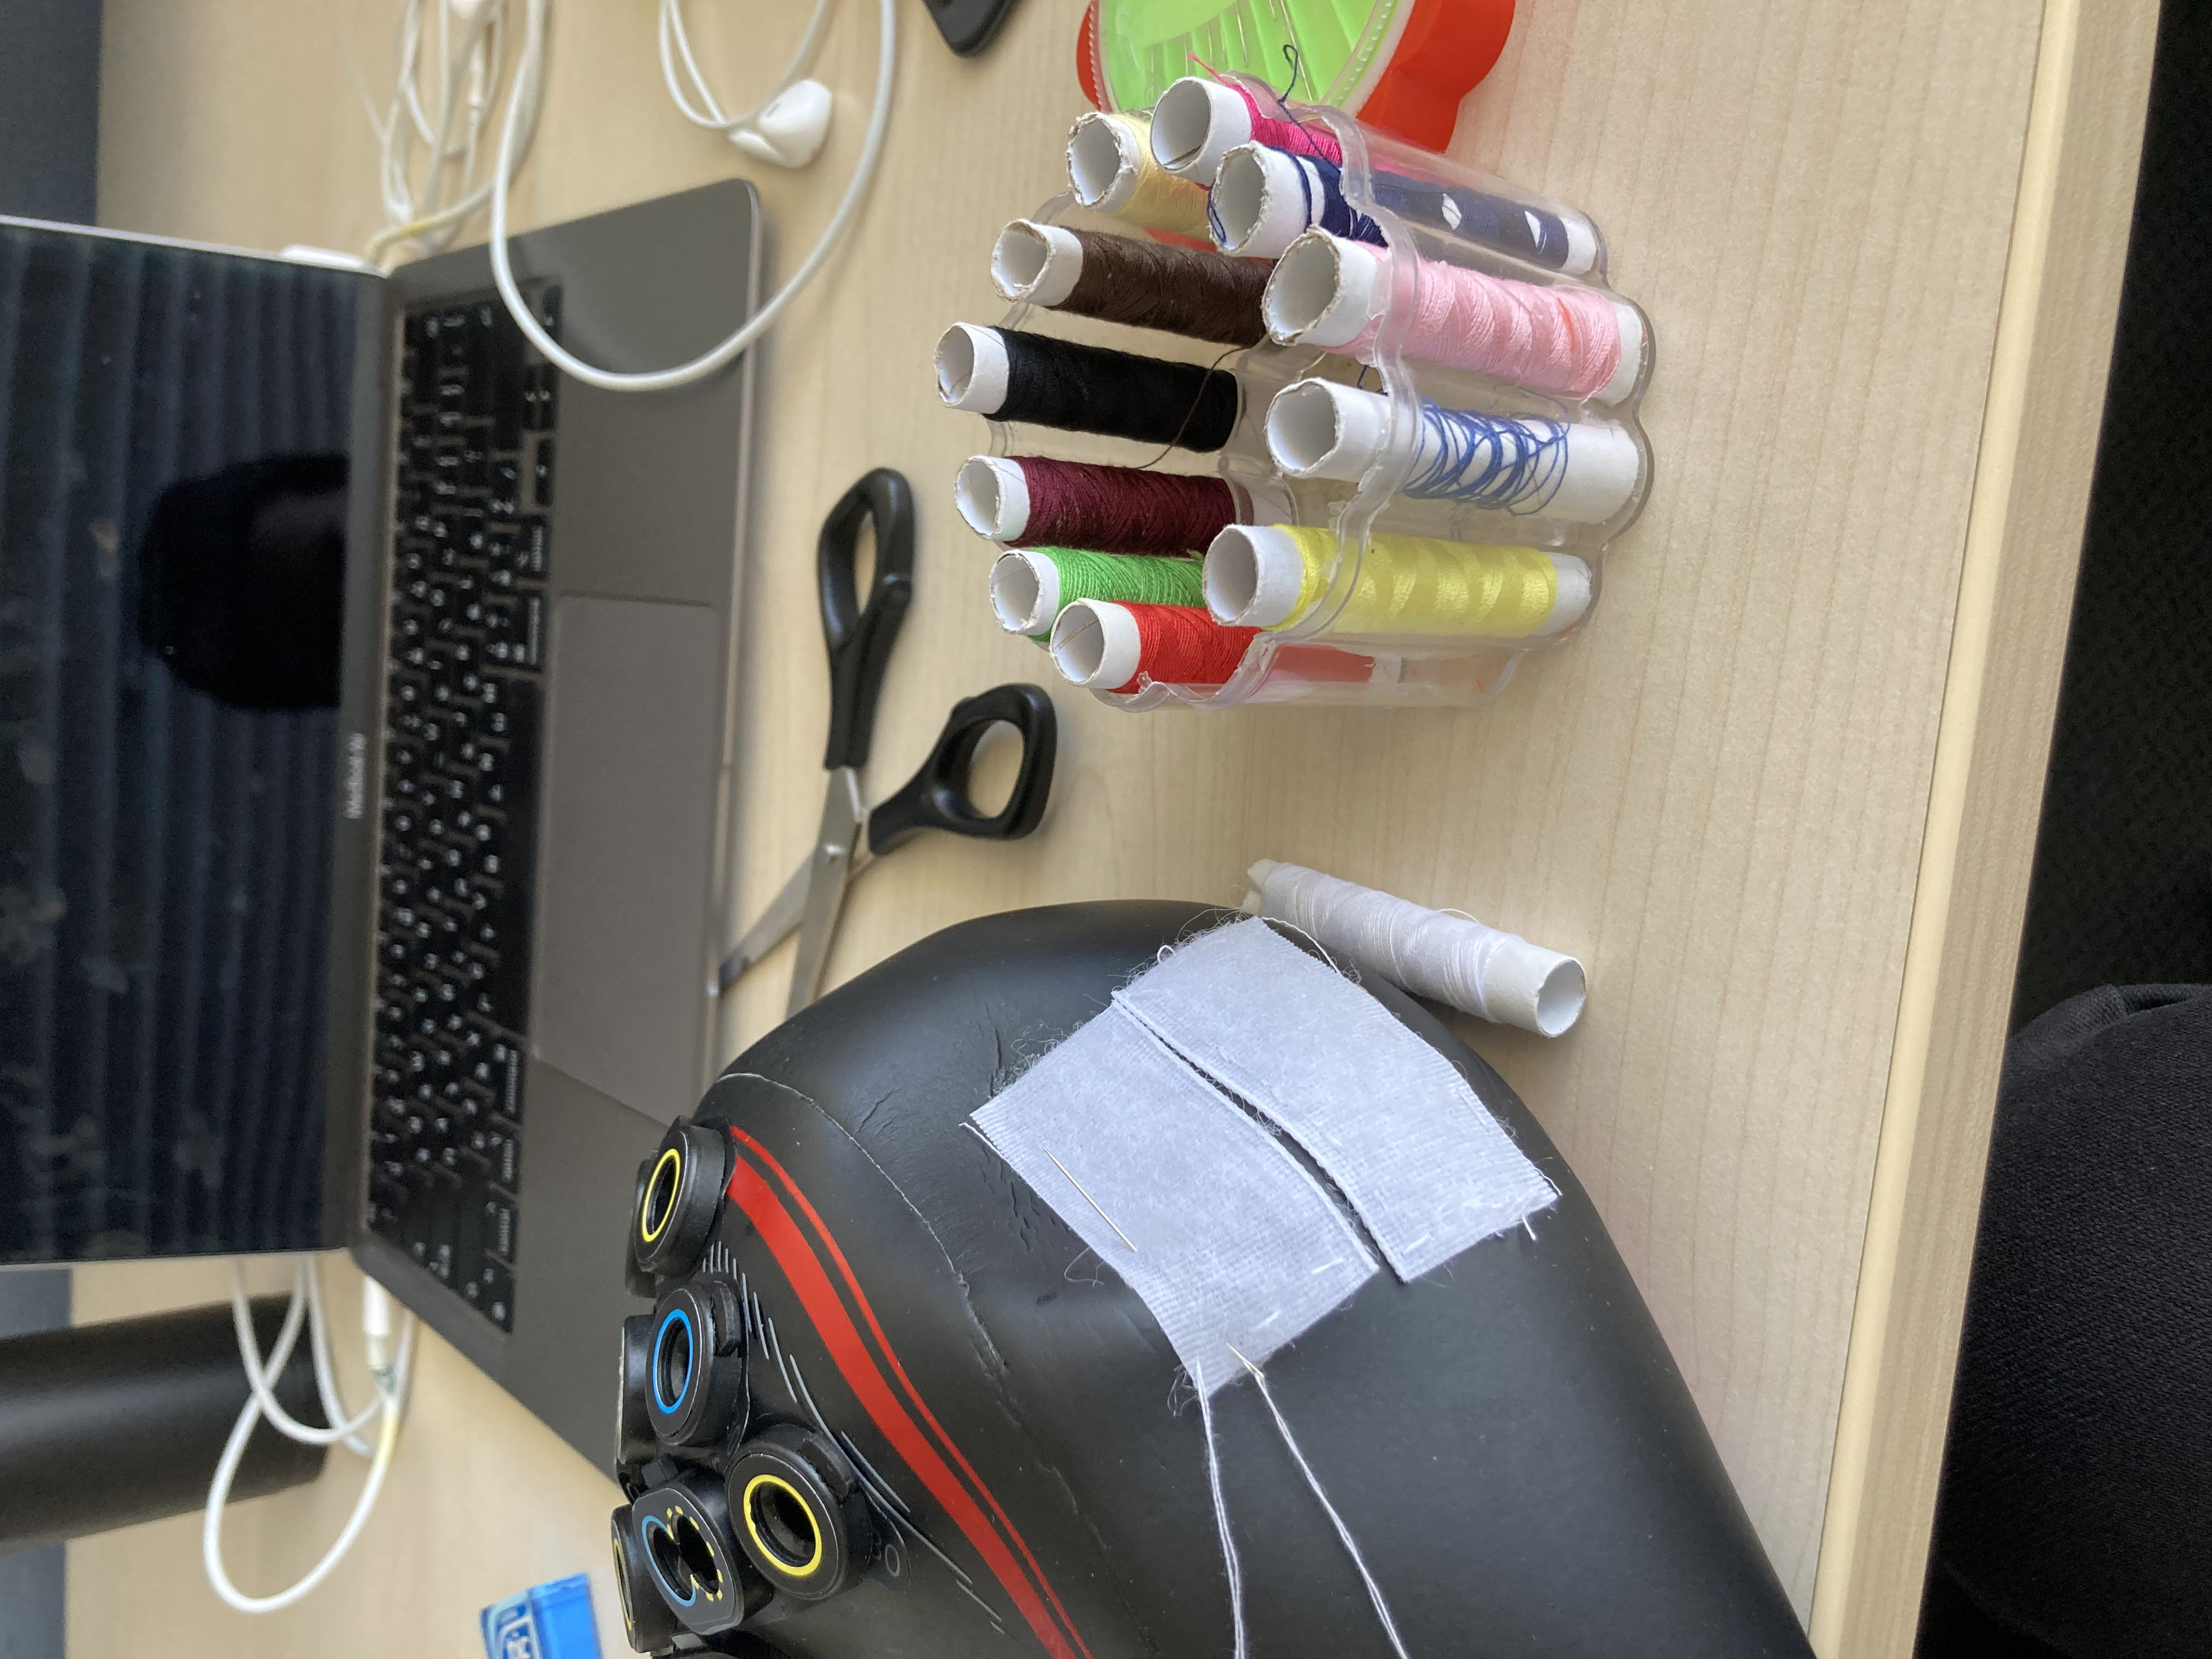
\includegraphics[scale= 0.05, angle= -90, origin= c]{bilder/IMG_9825.jpg}
  \caption{Manufacturing process of the cap}
  \label{fig:ManufactureCap}
\end{minipage} \hfill
\begin{minipage}[c]{.4\linewidth}
  \centering
  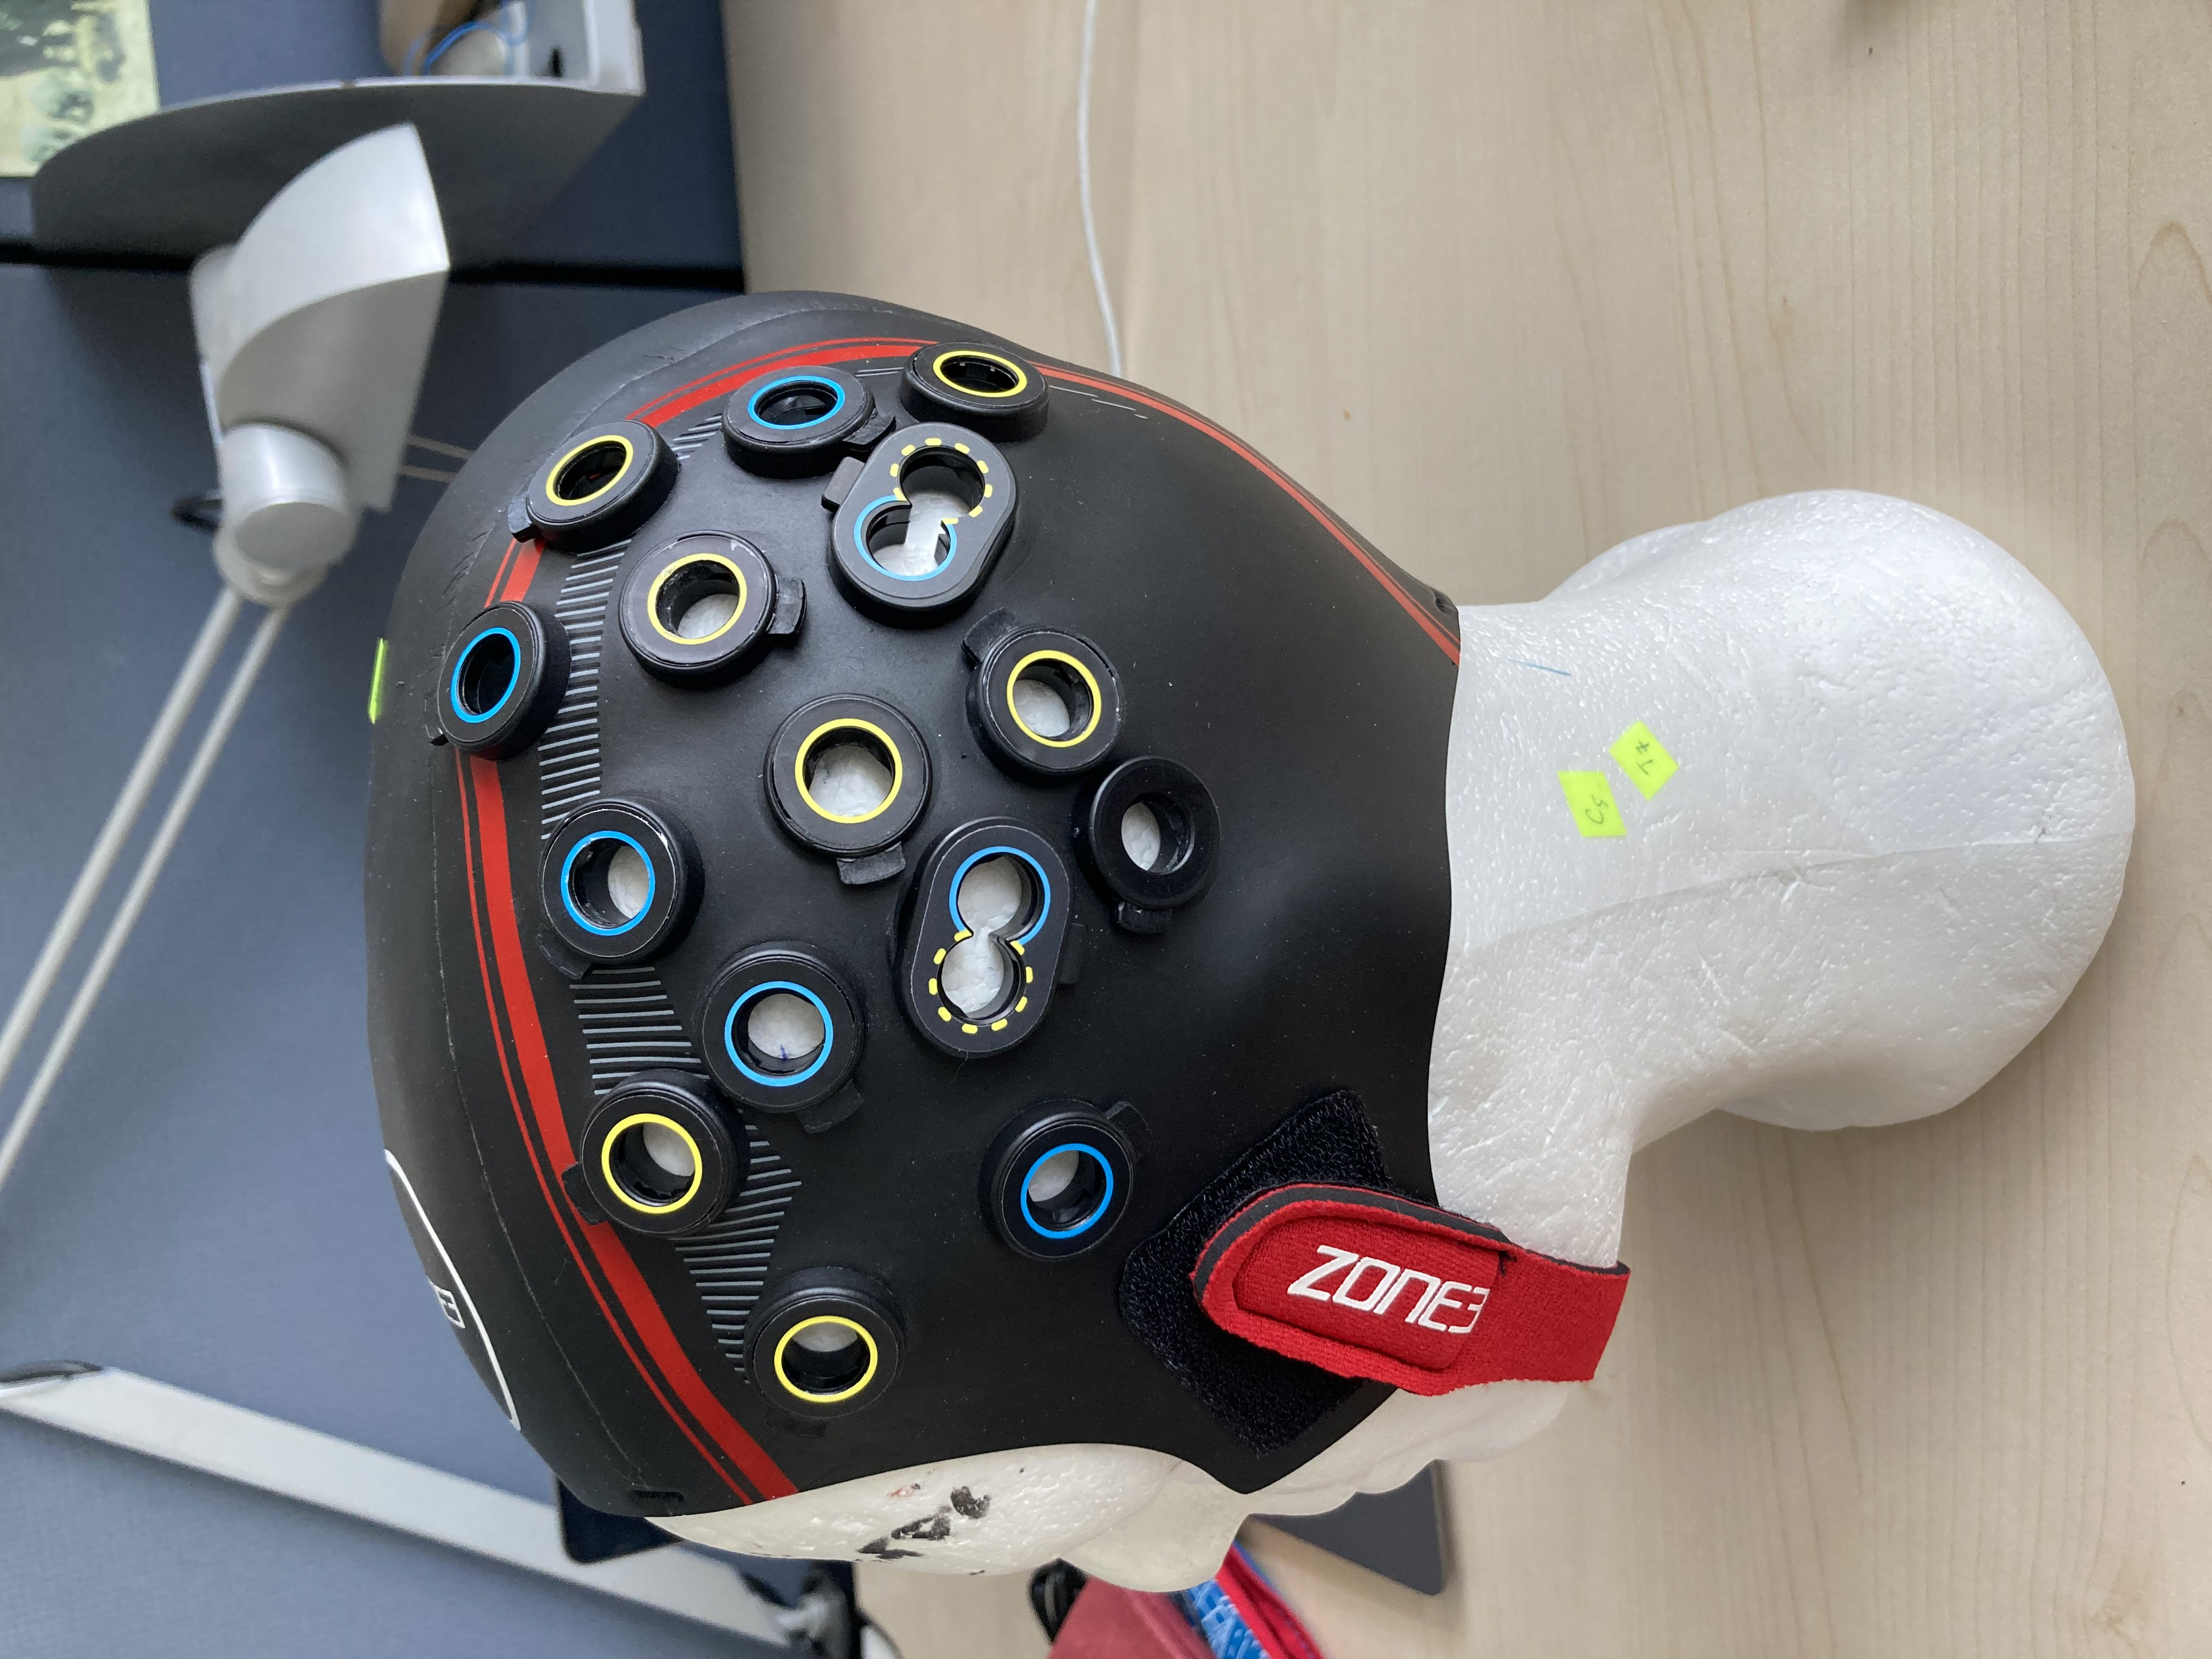
\includegraphics[scale= 0.05, angle= -90, origin= c] {bilder/IMG_9768.jpg}
  \caption{Finished cap on dummy}
  \label{fig:FinishedCap}
\end{minipage}
\end{figure}

Due to device limitations, we only measured one side of the brain. According to Frost et al. \citeyearpar {Frost1999-vs} , language processing has been predominantly associated to cortical activity in the left hemisphere. As a result, we decided to focus on the left hemisphere.

The fNIRS device we used also had limited number of sources and detectors. In the original design of Weder et al. \citeyearpar{Weder2018}, 9 sources and 9 detectors were used. However, the device we used had only 10 sources and 8 detectors. Hence, we shifted one channel around T7 a little bit to the left, so that one less detector is needed. At the end, there were 12 long channels and 2 short channels in out setup (see Figure ~\ref{fig:ChannelDef}).

The physical cap was self-made from a swimming cap (see Figure ~\ref {fig:FinishedCap} ~\ref {fig:ManufactureCap}). With the help of a dummy head model, correct positions of the optodes were marked and holes were drilled accordingly. The mounts were put on the cap on the holes. In order to ensure the correct channels length to be fixed exactly at 30 mm, plastic holders were also placed on the long channels. The Brite23 package comes with mounts for short channels. Thus, no plastic holders were needed in the case. The short channels were 11 mm long. The self-made cap turned out to work out well. The contacts between the scalp and the optodes were good thanks to the elastic characteristic of the material.



\section {Acoustic Stimulation during fNIRS Experiment}
Auditory stimuli were delivered binaurally via an audio metric headphone (Sennheiser HD 650) \footnote {\url{https://www.sennheiser-hearing.com/de-DE/p/hd-650/}}. Stimuli consisted of 20-s chunks of the \acrshort{icra} noise \footnote {The ICRA-Noise has been developed for the International Collegium of Rehabilitative Audiology by the HACTES work group (Hearing Aid Clinical Test Environment standardisation). The purpose was to establish collection of noise signals to be used as background noise in clinical tests of hearing aids and possibly for measuring characteristics of non-linear instruments. Source: \url{https://icra-audiology.org/Repository/icra-noise}} \citep {Dreschler}. 

To begin with, ICRA noise was developed to be used as background noise in clinical tests of hearing aids and possibly for measruing characteristics of non-linear instruments. The signals are based on live English speech from the EUROM database \citep {chanEUROM} in which a female speaker is explaining about the system of arithmetical notation. The speech signals were sampled with a sampling rate of 44.1 kHz. By composing the speech signals with well defined spectral and temporal characteristic, the modified signals have long-term spectrums but are completely unintelligible. 
 
We chose to use ICRA noise as stimuli based on several reasons. For one, ICRA noise is a broadband amplitude-modulated signal. By selecting a broadband stimulus, broad cortical auditory areas are activated more strongly compared to simple static stimulus, e.g. a pure tone with a fixed amplitude. The bandwidth of auditory stimuli is positively correlated with the mean percentage signal change and spread of cortical activation \citep {Hall}. A previous fMRI study also manifested that more complex auditory stimuli elicit greater response in most parts of the auditory cortex \citep {Belin2002}. For the other, ICRA noise is a well-known and accessible stimulus. It is also considered as an international de facto standard for hearing research. In this way, our results can be directly compared to other research.
 
As for choosing different sound level pressure, we picked 40 dB, 65 dB, 90 dB, and silent stimulus, i.e. 0 dB. Calibrations were performed using an oscilloscope, a G.R.A.S. Power Module Type 12AK \footnote {\url{https://www.grasacoustics.com/products/power-module/traditional-power-supply-lemo/product/225-12ak}},  and an artificial ear (G.R.A.S. 43AA) \footnote {\url {https://www.grasacoustics.com/products/ear-simulator-kit/traditional-power-supply-lemo/product/238-43aa}}. The artificial ear transform the sound pressure levels (\acrshort{spl}s) into electrical signals, i.e. voltages that can be measured by the oscilloscope. According to the instruction manual of the G.R.A.S. artificial ear, the measured level is 11.19 $[ \frac {mV}{Pa}]$. The SPL in dB is defined as 
\begin{equation}
SPL [dB] = 20 \cdot log \frac{P}{P_0} \text{ , where $P_0$ is $20 \mu$Pa}
\end{equation}
Hence, the relation between SPL and measured voltage should be.
\begin{equation}
V = 20{ \mu Pa} \cdot 10^{\frac {SPL}{20}}  \cdot 10^{\frac{Gain}{20}} \cdot 11.19 {\frac {mV}{Pa}} 
\end{equation}
The headphone with the artificial ear were setup together in the sound booth to ensure minimal environmental noise. The output voltages were measured with the oscilloscope. This way, the corresponding amplitude inputs for later MATLAB scripts for the desire SPLs can be determined.

MATLAB (version 2019b) and Oxysoft (version 3.3.33) were used during the measurement. In MATLAB, a chunk in the ICRA audio files was selected. It was multiplied with different amplitude levels for 4 SPLs and ramped with a 10-ms Hanning window. In each epoch, all four stimuli (0dB, 40 dB, 65 dB, and 90 dB) were played randomly once. After each stimulus, there was a 25-s silence rest to wait for the hemodynamic response. For each participant, 8 epochs were conducted. The stimuli were marked with \acrlong{lsl}s \footnote {The lab streaming layer (LSL) is a system for the unified collection of measurement time series in research experiments that handles both the networking, time-synchronization, (near-) real-time access as well as optionally the centralized collection, viewing and disk recording of the data. Source : \url{https://github.com/sccn/labstreaminglayer}} to note which SPL it was. This \acrlong {lsl} also acted as an interface between MATLAB and Oxysoft, so that Oxysoft could mark the time for each stimulus in the measurement data correctly in real time.

\section {fNIRS Setup}
The Brite23 \footnote {\url{https://neurolite.ch/sites/default/files/Brite23\%20Brochure_0.pdf}} was used as the fNIRS device in this research. It is light weight, has 10 sources and 8 detectors and can support up to 23 channels. The Brite23 fNIRS device was connected via bluetooth to the PC and the Oxysoft software. For each measurement, the DPF was calculated depending on the age of the participant. The sampling rate was fixed at 50 Hz, for enough resolution but not unnecessarily large in terms of data size.

After the settings in the Oxysoft software were done, the participant were asked to put on the self-made cap. On each optode position, the hair would be put aside gently with a Q-tip to ensure better contact between the optodes and the scalp. Then, the participants would be asked to put on the headphone and go into the sound-attenuating booth. The participants were also asked to keep the eyes closed and keep the head still to ensure minimum interference from visual stimulation and motion.


\section {Data preprocesing}
Data preprocessing and analysis was executed in MATLAB (Mathworks, USA) and the Homer3 toolbox. The following steps were executed.

\begin{figure}[H]
  \centering
    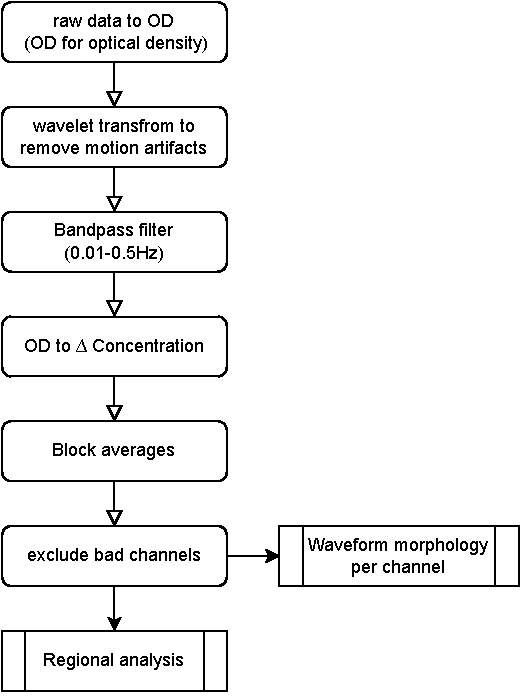
\includegraphics[scale=.9]{pdf/flowchart2.pdf}
  \caption{Flow chart of data processing}
  \label{fig:somesignal}
\end{figure}


First, the hemodynamic response was extracted with the Homer3 toolbox. Raw data were converted into optical densities. Motion artifacts were removed by using wavelet transformation of the data. \citep {Molavi_2012}. We also tried to use \acrlong{pca} (\acrshort{pca}) to remove motion artifact, since PCA has the advantage of faster computation. However, it is also known for tending to remove too much of the activation signal in adults. Wavelet transform on the other hand, takes longer to compute, but it is better at maintaining relevant frequency content. Then, the Homer3 toolbox bandpass filter (0.01 - 0.5 Hz) was used to reduced drift, broadband noise, heartbeat, and respiration artifacts. Changes of concentration of \acrlong{HbO} (\acrshort{HbO}) and  \acrlong{HbR} (\acrshort{HbR}) were estimated by applying the modified Beer-Lambert Law  \citep {Delpy_1988}. In this step, a correction factor, DPF, is used. Although strictly speaking, the DPF should be experimentally obtained with \acrshort{fd-nirs} or \acrshort{td-nirs}, due to device limitations, it was not possible in this project. Hence, in our research, the DPF was determined by wavelengths of the fNIRS device and age of the participant. \citep {Duncan1996MeasurementOC}. According to Duncan et al. \citeyearpar {Duncan1996MeasurementOC}, the DPF for two wavelengths can be calculated with the formulae:
\begin{equation}
DPF_{744} = 5.11 + 0.106 \cdot Age^{0.723}
\end{equation}

\begin{equation}
DPF_{852} = 4.67 + 0.062 \cdot Age^{0.819}
\end{equation}

\noindent with age given in years.\\
 
Duncan et al. \citeyearpar{Duncan1996MeasurementOC} developed a broadband radiofrequency-modulated \acrlong{prs} (\acrshort{prs}) instrument using four wavelengths(690, 744, 807, and 832 nm) which can measure phase shifts through more than 4 cm of brain tissue in less than one second. In the study, the modulation frequency was set at 200 MHz, which has been shown theoretically to be a frequency at which phase shift and true mean optical path length are equal \citep {Arridge_1992}. By dividing the true mean optical path length with source detector  separation, the DPF can be obtained. 

The authors also provided mathematical models based on the measurements. The estimated DPF is in a sequential order as the used wavelengths. The shorter the wavelength, the larger the mean DPF they measured. Even though only four equations were provided with the above-mentioned four wavelengths, and our wavelengths were different then that of the authors used, we were convinced that with the above two equations, we could still get fair estimate of the true DPF in our case.

\begin{figure}[H]
  \centering
    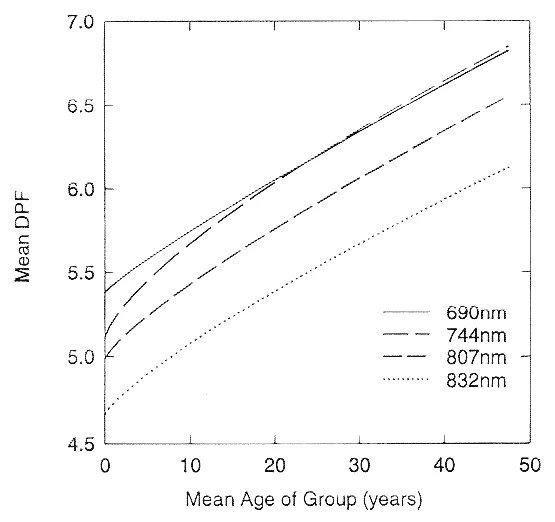
\includegraphics[scale=.45]{bilder/fig3_duncan.jpg}
  \caption{Age dependence of DPF. Taken rom Duncan et al. \citeyearpar{Duncan1996MeasurementOC} }
  \label{fig:somesignal}
\end{figure}

It is important to note that the noise due to motion artifacts, drift, broadband noise, heartbeat, and respiration artifacts need to be processed before the concentration was estimated, according to the previous research \citep {Huppert:09}.

Later on, the extracerrebral component in long channels should be reduced by using measurements from the short channels as follows: the first principal components from the two short channels were estimated and then multiplied by its coefficient from the \acrlong{glm} (\acrshort {glm}) \citep{friston1994statistical}. However, this was not done in the present study, since the coefficient from the GLM were very small. They were of the magnitudes $10^{-16}$ , whereas the hemodynamic response in the long channels were of the magnitudes $10^{-5}$. Hence, we concluded the extracerebral components in our case could be negligible.

Channels with unusable data were excluded here for further analysis. The \acrlong{sci} (\acrshort{sci}) \citep {Pollonini2013} is a common measure to detect unusable channels . The SCI estimates the correlation between the two wavelength channels in the cardiac band as the follows.

First, the signal is bandpass-filtered to keep only the cardiac band. In our case, a wide band of (0.5 - 2.5) Hz was chosen. Then, amplitude normalization is performed, and the SCI computation is defined as the absolute cross-correlation value at zero-time lag \citep {Pollonini2013}.


\begin{figure}[H]
  \centering
    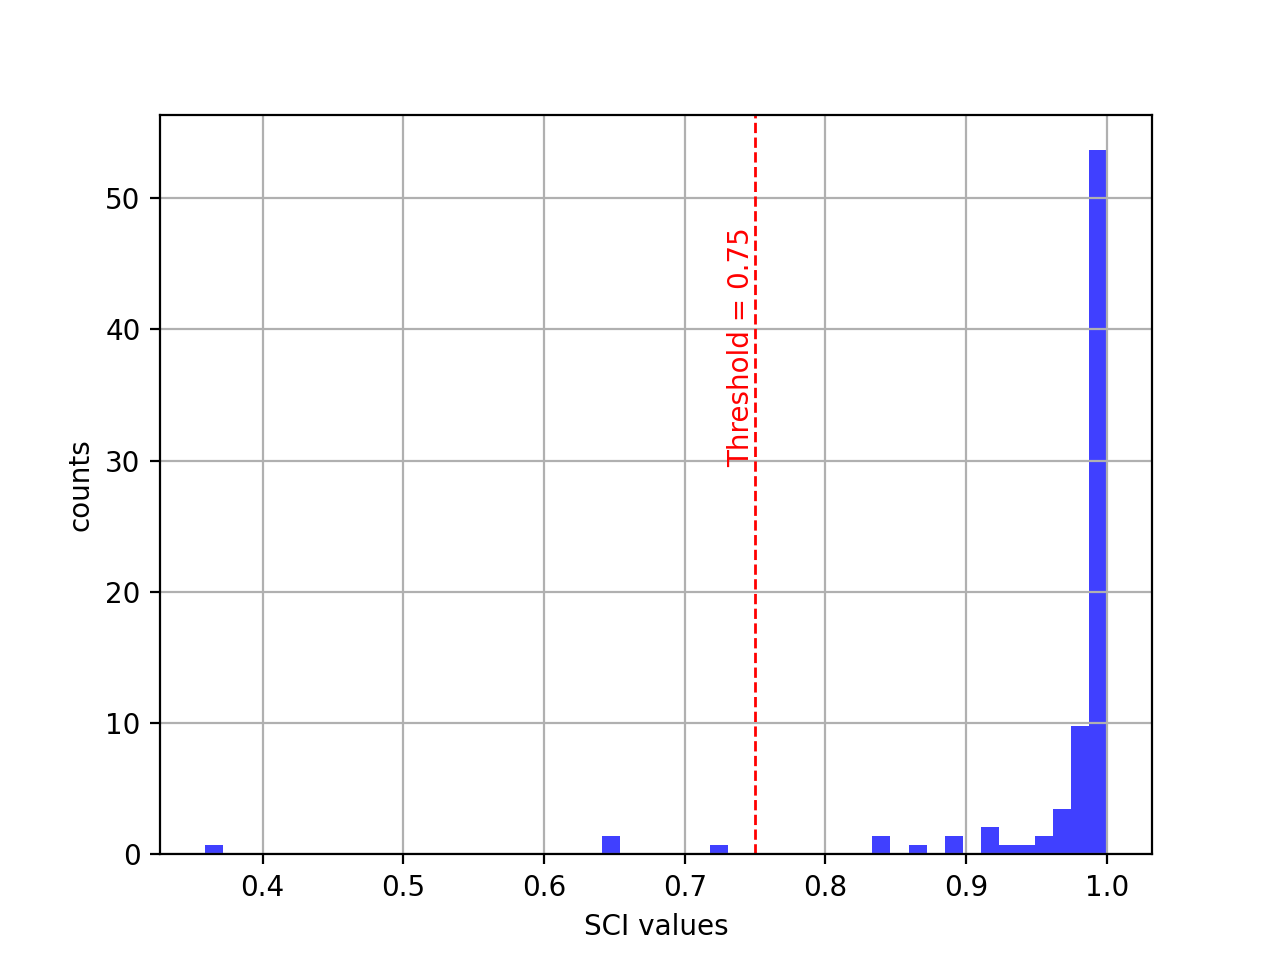
\includegraphics[scale=.75]{bilder/SCI_hist.png}
  \caption{Distribution of SCI values.}
   \label{fig:somesignal}
    \medskip
     \small {In the present study, only four channels failed to reach the threshold of 0.75. In other words, of all the measurements (14 channels per participant, 8 participants in total). Over 96\% of the measurements passed the SCI threshold.}
 
\end{figure}




